\documentclass[tikz,border=6pt]{standalone}
\usetikzlibrary{arrows.meta}
\definecolor{red}{HTML}{A50F2D}\definecolor{ink}{HTML}{141414}\definecolor{gry}{HTML}{5F5F5F}\definecolor{blu}{HTML}{1F5F99}\definecolor{gn}{HTML}{1B7F5F}
\begin{document}
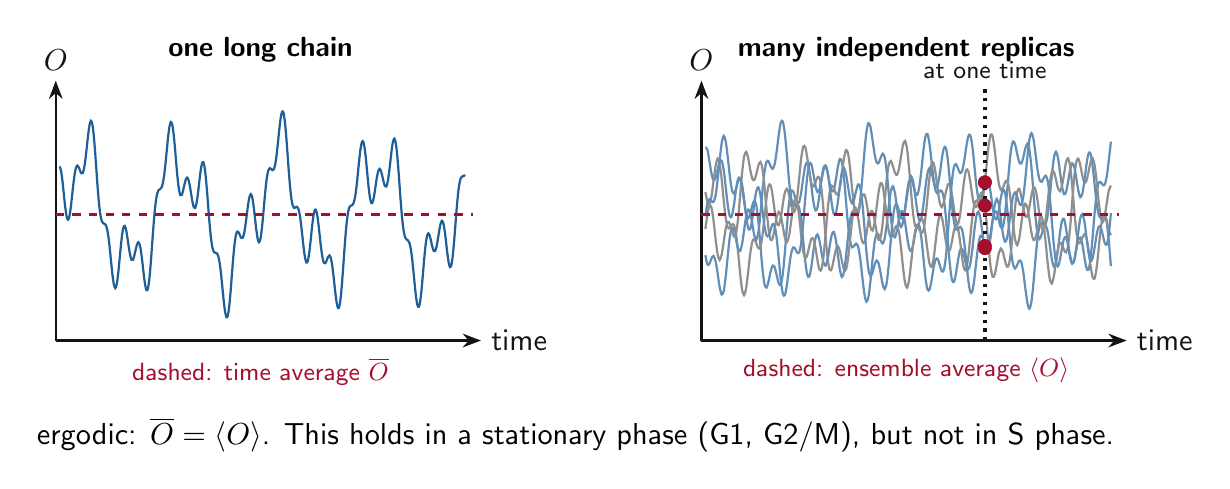
\begin{tikzpicture}[font=\sffamily\fontsize{11}{13}\selectfont,>=Stealth]
% left: one long chain
\node[font=\sffamily\bfseries] at (2.6,3.7) {one long chain};
\draw[->,ink,thick] (0,0)--(5.4,0) node[right]{time};
\draw[->,ink,thick] (0,0)--(0,3.3) node[above]{$O$};
\draw[blu,thick,smooth,samples=300,domain=0.05:5.2] plot (\x,{1.6+0.7*sin(deg(5*\x))+0.4*sin(deg(13*\x+2))+0.25*sin(deg(31*\x))});
\draw[red,very thick,dashed] (0,1.6)--(5.3,1.6);
\node[red,anchor=north,font=\sffamily\small] at (2.6,-0.1) {dashed: time average $\overline{O}$};
% right: many replicas
\begin{scope}[xshift=8.2cm]
\node[font=\sffamily\bfseries] at (2.6,3.7) {many independent replicas};
\draw[->,ink,thick] (0,0)--(5.4,0) node[right]{time};
\draw[->,ink,thick] (0,0)--(0,3.3) node[above]{$O$};
\foreach \p/\a/\c in {0.3/0.6/blu,1.7/0.5/gry,3.1/0.7/blu,4.5/0.4/gry,5.9/0.55/blu}{
 \draw[\c!70,thick,smooth,samples=200,domain=0.05:5.2] plot (\x,{1.6+\a*sin(deg(5*\x+\p))+0.3*sin(deg(11*\x+3*\p))+0.25*sin(deg(29*\x+\p))});}
\draw[ink,dotted,very thick] (3.6,0)--(3.6,3.2);
\foreach \p/\a in {0.3/0.6,1.7/0.5,3.1/0.7,4.5/0.4,5.9/0.55}{\fill[red] (3.6,{1.6+\a*sin(deg(5*3.6+\p))+0.3*sin(deg(11*3.6+3*\p))+0.25*sin(deg(29*3.6+\p))}) circle (2.5pt);}
\draw[red,very thick,dashed] (0,1.6)--(5.3,1.6);
\node[red,anchor=north,font=\sffamily\small] at (2.6,-0.1) {dashed: ensemble average $\langle O\rangle$};
\node[ink,font=\sffamily\small,anchor=south] at (3.6,3.2) {at one time};
\end{scope}
\node[align=center,font=\sffamily\fontsize{11}{13}\selectfont] at (6.6,-1.2) {ergodic: $\overline{O} = \langle O\rangle$. This holds in a stationary phase (G1, G2/M), but not in S phase.};
\end{tikzpicture}
\end{document}
